\documentclass[11pt]{article}

% --- packages (kept to widely-available ones for clean compilation) ---
\usepackage[utf8]{inputenc}
\usepackage[T1]{fontenc}
\usepackage[a4paper,margin=2.2cm]{geometry}
\usepackage{graphicx}
\usepackage{amssymb}
\usepackage{xcolor}
\usepackage{enumitem}
\usepackage{booktabs}
\usepackage{fancyhdr}
\usepackage{titlesec}
\usepackage[hidelinks]{hyperref}
\usepackage{parskip}

% --- colours ---
\definecolor{leafgreen}{RGB}{60,150,70}
\definecolor{darkgreen}{RGB}{34,90,40}
\definecolor{tokengold}{RGB}{214,158,46}
\definecolor{lossbrown}{RGB}{120,94,80}
\definecolor{rainblue}{RGB}{120,170,210}
\definecolor{boxbg}{RGB}{240,248,240}
\definecolor{boxedge}{RGB}{60,150,70}
\definecolor{warnbg}{RGB}{251,243,233}
\definecolor{warnedge}{RGB}{214,158,46}
\definecolor{inkgrey}{RGB}{90,90,90}

% --- headings ---
\titleformat{\section}{\Large\bfseries\color{darkgreen}}{\thesection.}{0.5em}{}
\titleformat{\subsection}{\large\bfseries\color{leafgreen}}{}{0em}{}

% --- header / footer ---
\pagestyle{fancy}
\fancyhf{}
\lhead{\small\color{inkgrey}Fertilizer Game --- Farmer Guide}
\rhead{\small\color{inkgrey}CIMMYT}
\cfoot{\small\color{inkgrey}\thepage}
\renewcommand{\headrulewidth}{0.3pt}

% --- helper: a framed screenshot with a caption line ---
\newcommand{\screenshot}[2]{%
  \begin{center}
  \setlength{\fboxsep}{0pt}\setlength{\fboxrule}{0.6pt}%
  \fcolorbox{black!25}{white}{\includegraphics[width=0.92\linewidth]{#1}}\\[2pt]
  {\small\itshape\color{inkgrey}#2}
  \end{center}}

% --- helper: a "key idea" callout box (no extra packages needed) ---
\newcommand{\keybox}[2]{%
  \par\medskip\noindent
  \setlength{\fboxsep}{10pt}\setlength{\fboxrule}{1pt}%
  \fcolorbox{boxedge}{boxbg}{%
    \parbox{\dimexpr\linewidth-2\fboxsep-2\fboxrule\relax}{%
      {\bfseries\color{darkgreen}#1}\par\smallskip #2}}%
  \par\medskip}
\newcommand{\warnbox}[2]{%
  \par\medskip\noindent
  \setlength{\fboxsep}{10pt}\setlength{\fboxrule}{1pt}%
  \fcolorbox{warnedge}{warnbg}{%
    \parbox{\dimexpr\linewidth-2\fboxsep-2\fboxrule\relax}{%
      {\bfseries\color{tokengold}#1}\par\smallskip #2}}%
  \par\medskip}

\newcommand{\profit}[1]{\textbf{\color{leafgreen}#1}}
\newcommand{\loss}[1]{\textbf{\color{lossbrown}#1}}

\begin{document}

% ===================== TITLE =====================
\begin{titlepage}
\centering
\vspace*{2.5cm}
{\Huge\bfseries\color{darkgreen} The Fertilizer Game}\\[6pt]
{\Large\color{leafgreen} A Step-by-Step Guide for Farmers}\\[1.2cm]
{\large How to play, and what it teaches about using fertilizer\\ when the rain and the market price are uncertain}\\[2.2cm]
\setlength{\fboxsep}{0pt}\setlength{\fboxrule}{0.6pt}%
\fcolorbox{black!20}{white}{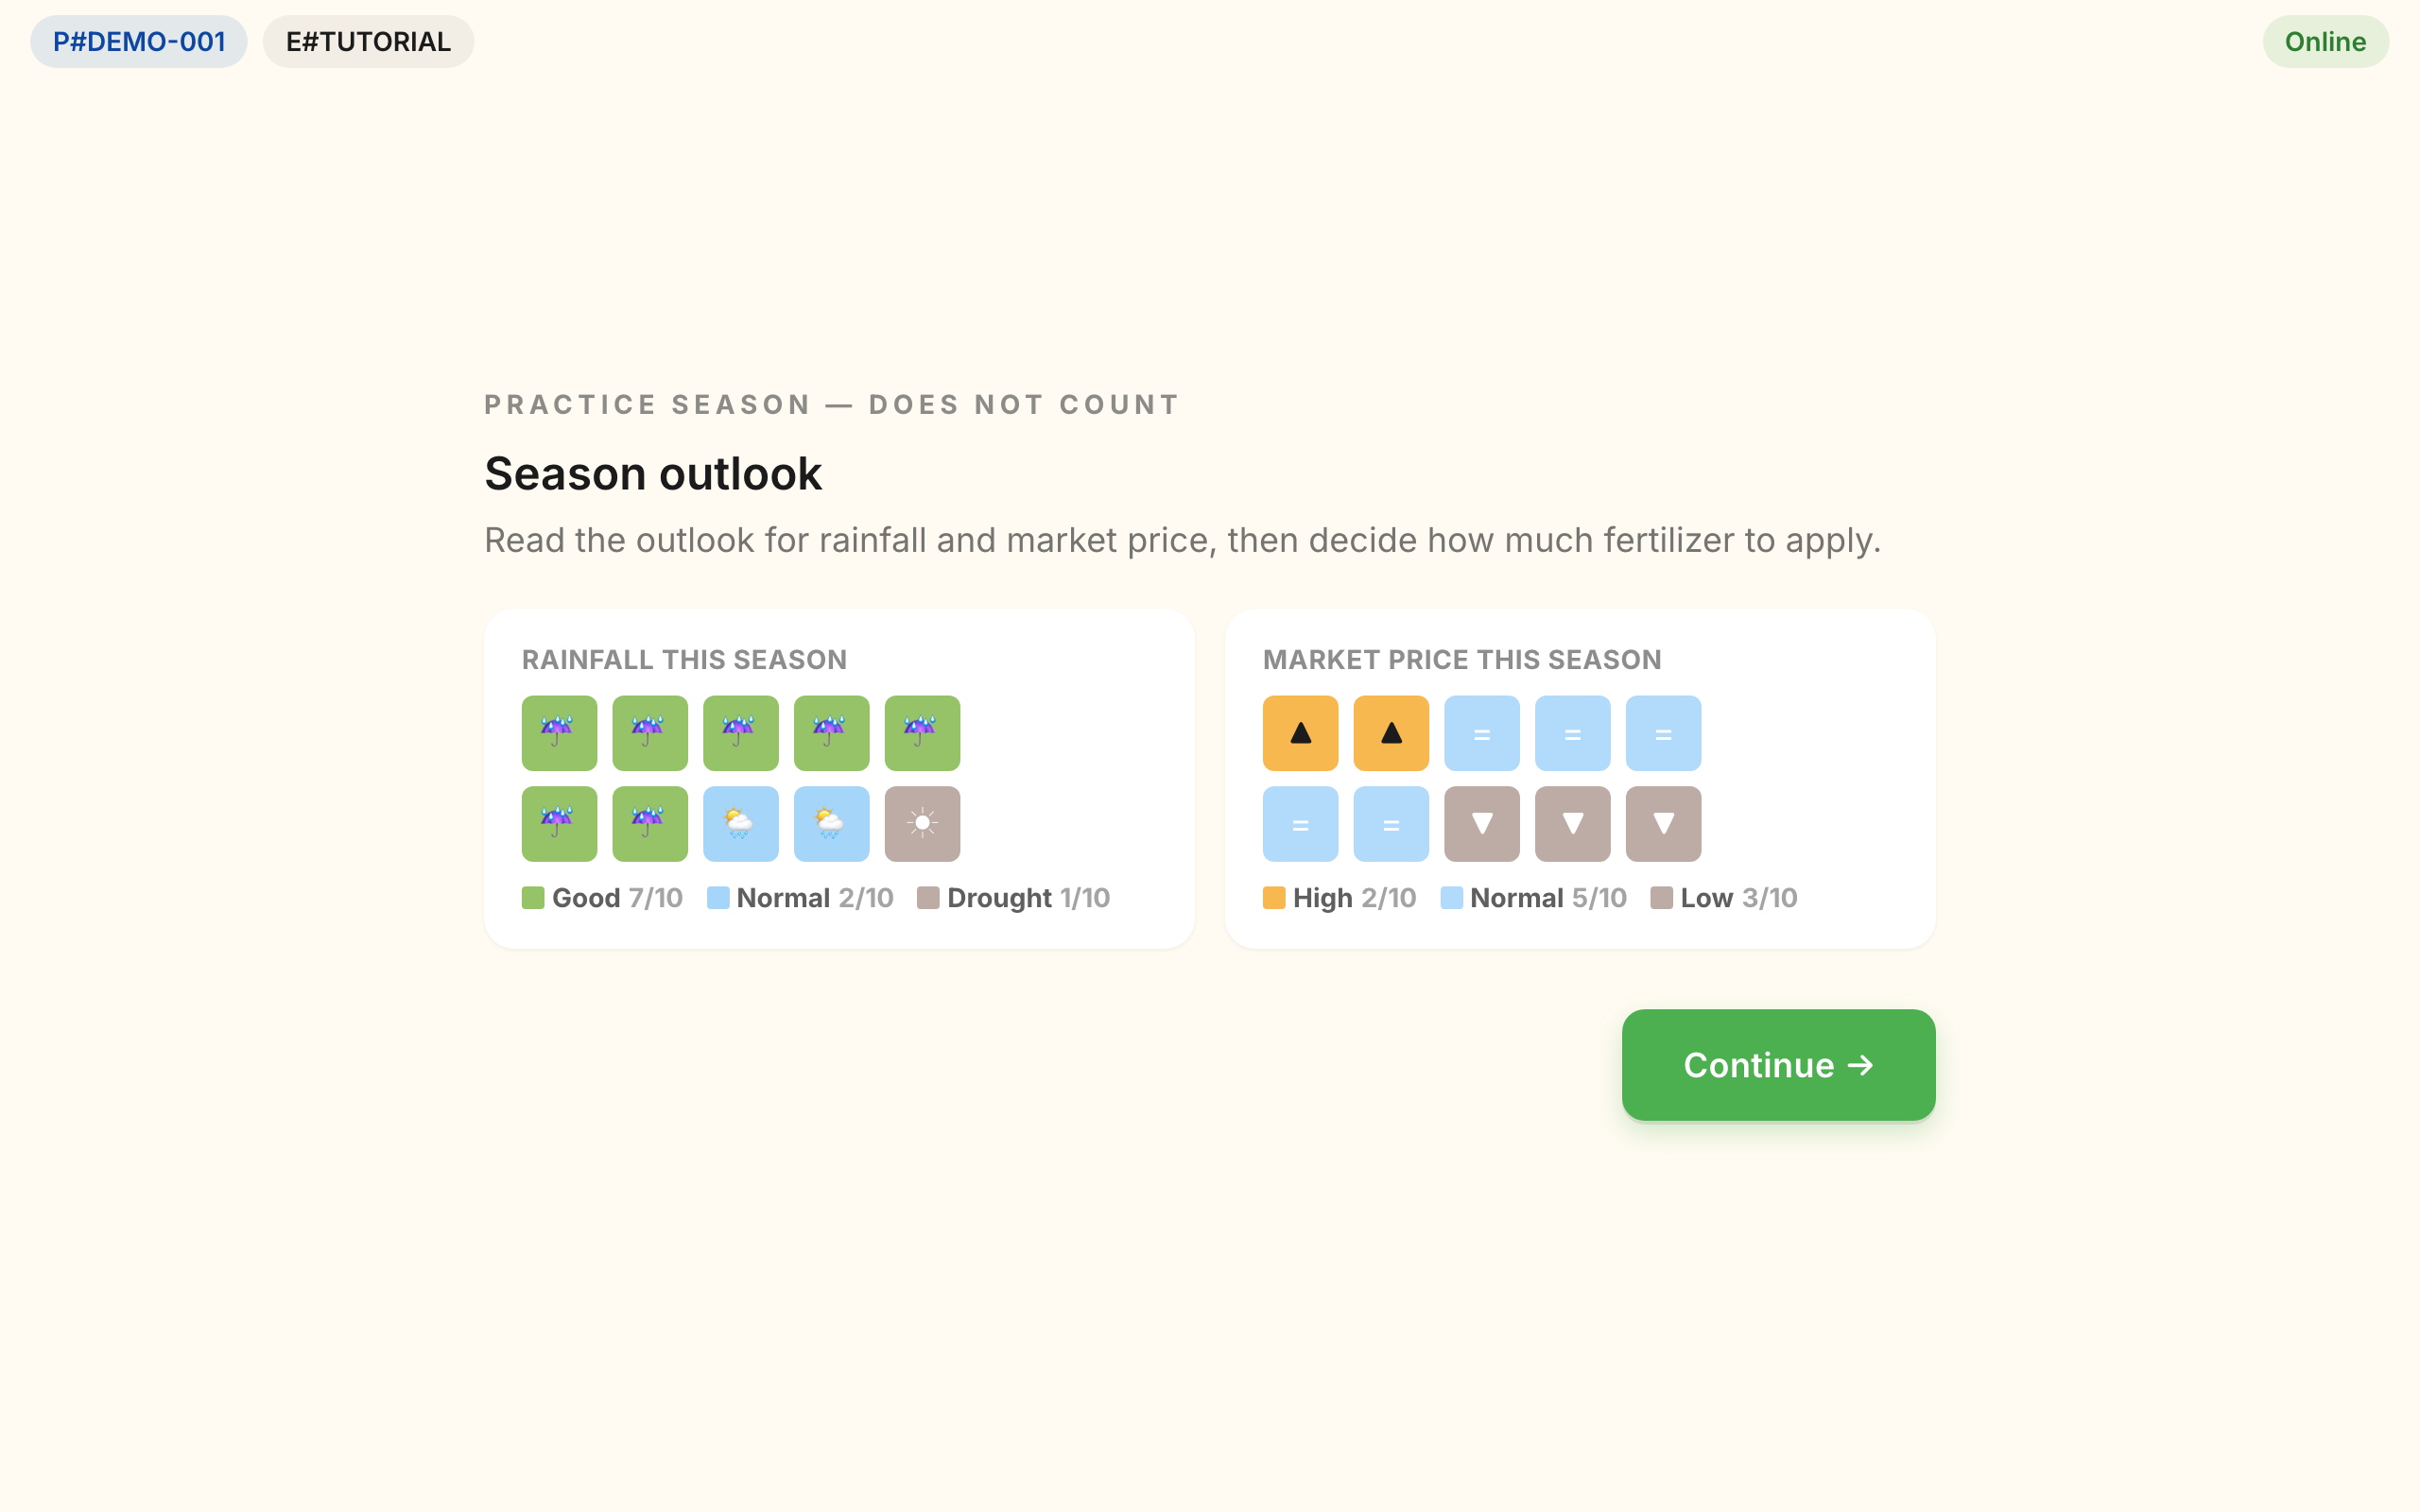
\includegraphics[width=0.8\linewidth]{img/08-briefing.png}}\\[2cm]
{\large\color{inkgrey} CIMMYT Field Experiment Tool}\\[2pt]
{\small\color{inkgrey} Maize $\cdot$ Nigeria $\cdot$ English / Hausa}
\vfill
{\small\color{inkgrey} This is a practice game played on a tablet. The money is play-money (\emph{tokens}); at the end your tokens are changed into real Naira.}
\end{titlepage}

% ===================== 1. WHAT IS THIS =====================
\section{What is this game about?}

In this game \textbf{you are a maize farmer}. Each \textbf{season} you must make one decision:
\textbf{how much fertilizer to buy for your field}.

The catch is that two things are \textbf{uncertain}, just like in real farming:
\begin{itemize}[leftmargin=1.4em]
  \item \textbf{The rain.} It can be \textbf{good}, \textbf{normal}, or there can be a \textbf{drought}.
  Fertilizer only helps your maize grow when there is enough water. In a drought, fertilizer does almost nothing.
  \item \textbf{The market price.} When you sell your maize the price can be \textbf{high}, \textbf{normal (mid)},
  or \textbf{low}. A good harvest is worth less money when the price is low.
\end{itemize}

Before each season the game \emph{tells you the chances} of good rain, drought, high price, and so on. Your
job is to look at those chances and decide how much fertilizer is worth buying.

\keybox{The one thing to remember}{%
Fertilizer is like an \textbf{investment}: you spend some of your money on it, hoping the extra harvest
will be worth \emph{more} than what you spent. Sometimes it pays off well. Sometimes ---
in a drought, or when the price is low --- it does not, and you \textbf{lose} the money you spent on it.
Buying \emph{no} fertilizer is always safe: you simply keep your money.}

% ===================== 2. WHAT YOU START WITH =====================
\section{What you start with each season}

At the start of \textbf{every} season you are given \textbf{25 tokens} (think of tokens as money).
\begin{itemize}[leftmargin=1.4em]
  \item Each \textbf{bag of fertilizer} costs \textbf{1 token}.
  \item You can buy from \textbf{0} bags (none) up to \textbf{10} bags.
  \item Any tokens you do \textbf{not} spend, you \textbf{keep}.
\end{itemize}

So if you buy 4 bags, you spend 4 tokens and keep 21. Those 4 bags are your \textbf{investment} ---
their job is to grow extra maize that you can sell.

There is \textbf{1 practice season} first (it does not count), and then \textbf{10 real seasons}.
Your tokens from the 10 real seasons are added up and changed into real money at the end.

% ===================== 3. ONE SEASON STEP BY STEP =====================
\section{One season, step by step}

Every season has the same five steps.

\subsection{Step 1 --- See the outlook (the chances)}

First you see the \textbf{chances} for this season: one picture for the \textbf{rain} and one for the
\textbf{market price}. Each picture has \textbf{10 small squares} that stand for 10 possible seasons.

\screenshot{img/08-briefing.png}{The season outlook. \textbf{Left:} rainfall --- here 7 of 10 squares are
Good (green), 2 Normal (blue), 1 Drought (grey). \textbf{Right:} market price --- 2 of 10 High, 5 Normal, 3 Low.}

How to read it: in the example above, \textbf{7 out of 10} squares show good rain, so good rain is
\emph{very likely} this season. Only \textbf{1 out of 10} shows drought, so a drought is \emph{unlikely}.
The more green squares, the safer it is to buy fertilizer.

\keybox{Reading the pictures}{%
\begin{tabular}{@{}ll@{}}
\textcolor{leafgreen}{$\blacksquare$} \textbf{Rain --- Good} & the best case; fertilizer works very well\\
\textcolor{rainblue}{$\blacksquare$} \textbf{Rain --- Normal} & fertilizer works, but less than in good rain\\
\textcolor{lossbrown}{$\blacksquare$} \textbf{Rain --- Drought} & fertilizer does \textbf{nothing}; you lose what you spent\\[4pt]
\textcolor{tokengold}{$\blacktriangle$} \textbf{Price --- High} & your maize sells for the most\\
\textcolor{rainblue}{$=$} \textbf{Price --- Normal} & a middle price\\
\textcolor{lossbrown}{$\blacktriangledown$} \textbf{Price --- Low} & your maize sells for little\\
\end{tabular}}

\subsection{Step 2 --- Decide how much fertilizer}

Now you choose your number of bags with the \textbf{minus ($-$)} and \textbf{plus ($+$)} buttons.
As you change it, you can see how many tokens you are keeping (``Tokens saved''). The rain and price
chances stay on the screen so you can keep looking at them while you decide.

\screenshot{img/09-dose.png}{Choosing the dose. Here 6 bags are selected. The card on the left shows the
tokens you would keep. Tap \textbf{Invest} when you are happy with your choice.}

\subsection{Step 3 --- Confirm (you cannot change it later)}

Once you tap Invest, the game asks you to confirm. \textbf{After you confirm you cannot change your decision}
--- just like in real life, once you have bought and applied the fertilizer, you cannot take it back.

\screenshot{img/10-confirm.png}{The confirmation. Tap \textbf{Go back} to change your mind, or
\textbf{Yes, invest in fertilizer} to lock in your decision.}

\subsection{Step 4 --- See what happened}

Now the season plays out. First the \textbf{rain} result is shown, then the \textbf{market price}.
This is decided by chance, using the odds you saw in Step~1 --- nobody can change it.

\begin{center}
\begin{minipage}{0.49\linewidth}\centering
\setlength{\fboxsep}{0pt}\setlength{\fboxrule}{0.6pt}%
\fcolorbox{black!25}{white}{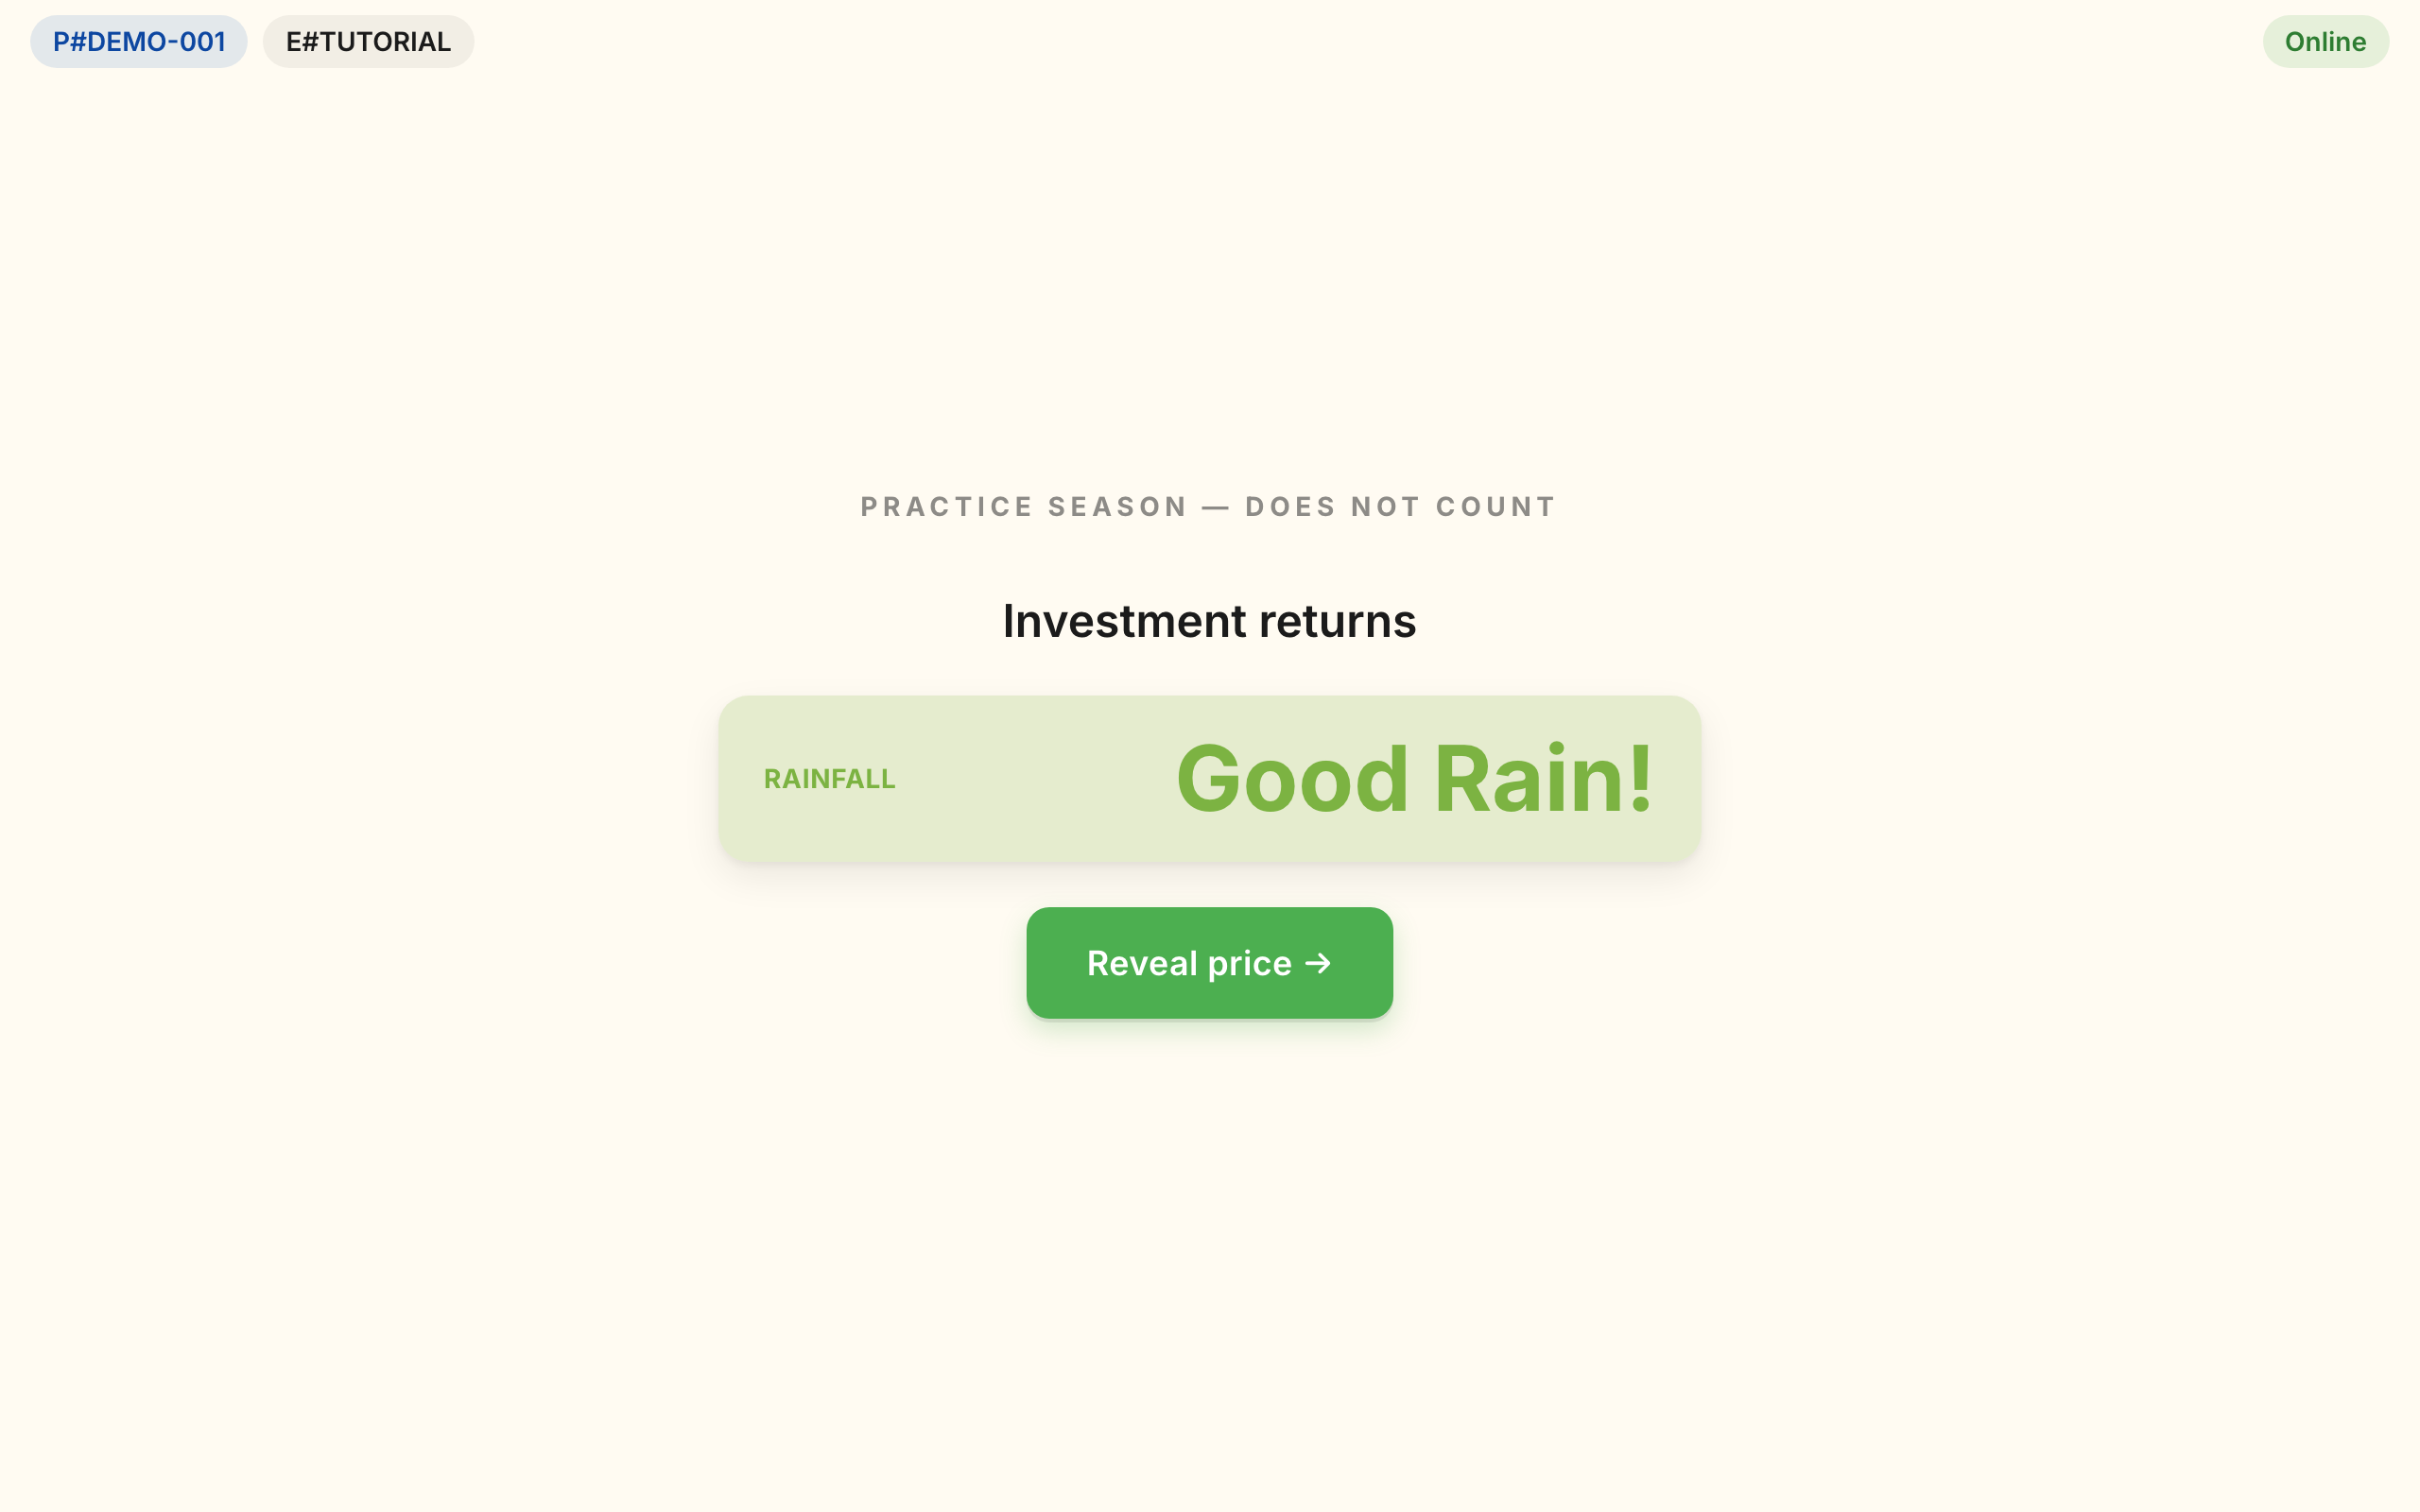
\includegraphics[width=\linewidth]{img/11-reveal-rain.png}}\\[2pt]
{\small\itshape\color{inkgrey} First: the rain result.}
\end{minipage}\hfill
\begin{minipage}{0.49\linewidth}\centering
\setlength{\fboxsep}{0pt}\setlength{\fboxrule}{0.6pt}%
\fcolorbox{black!25}{white}{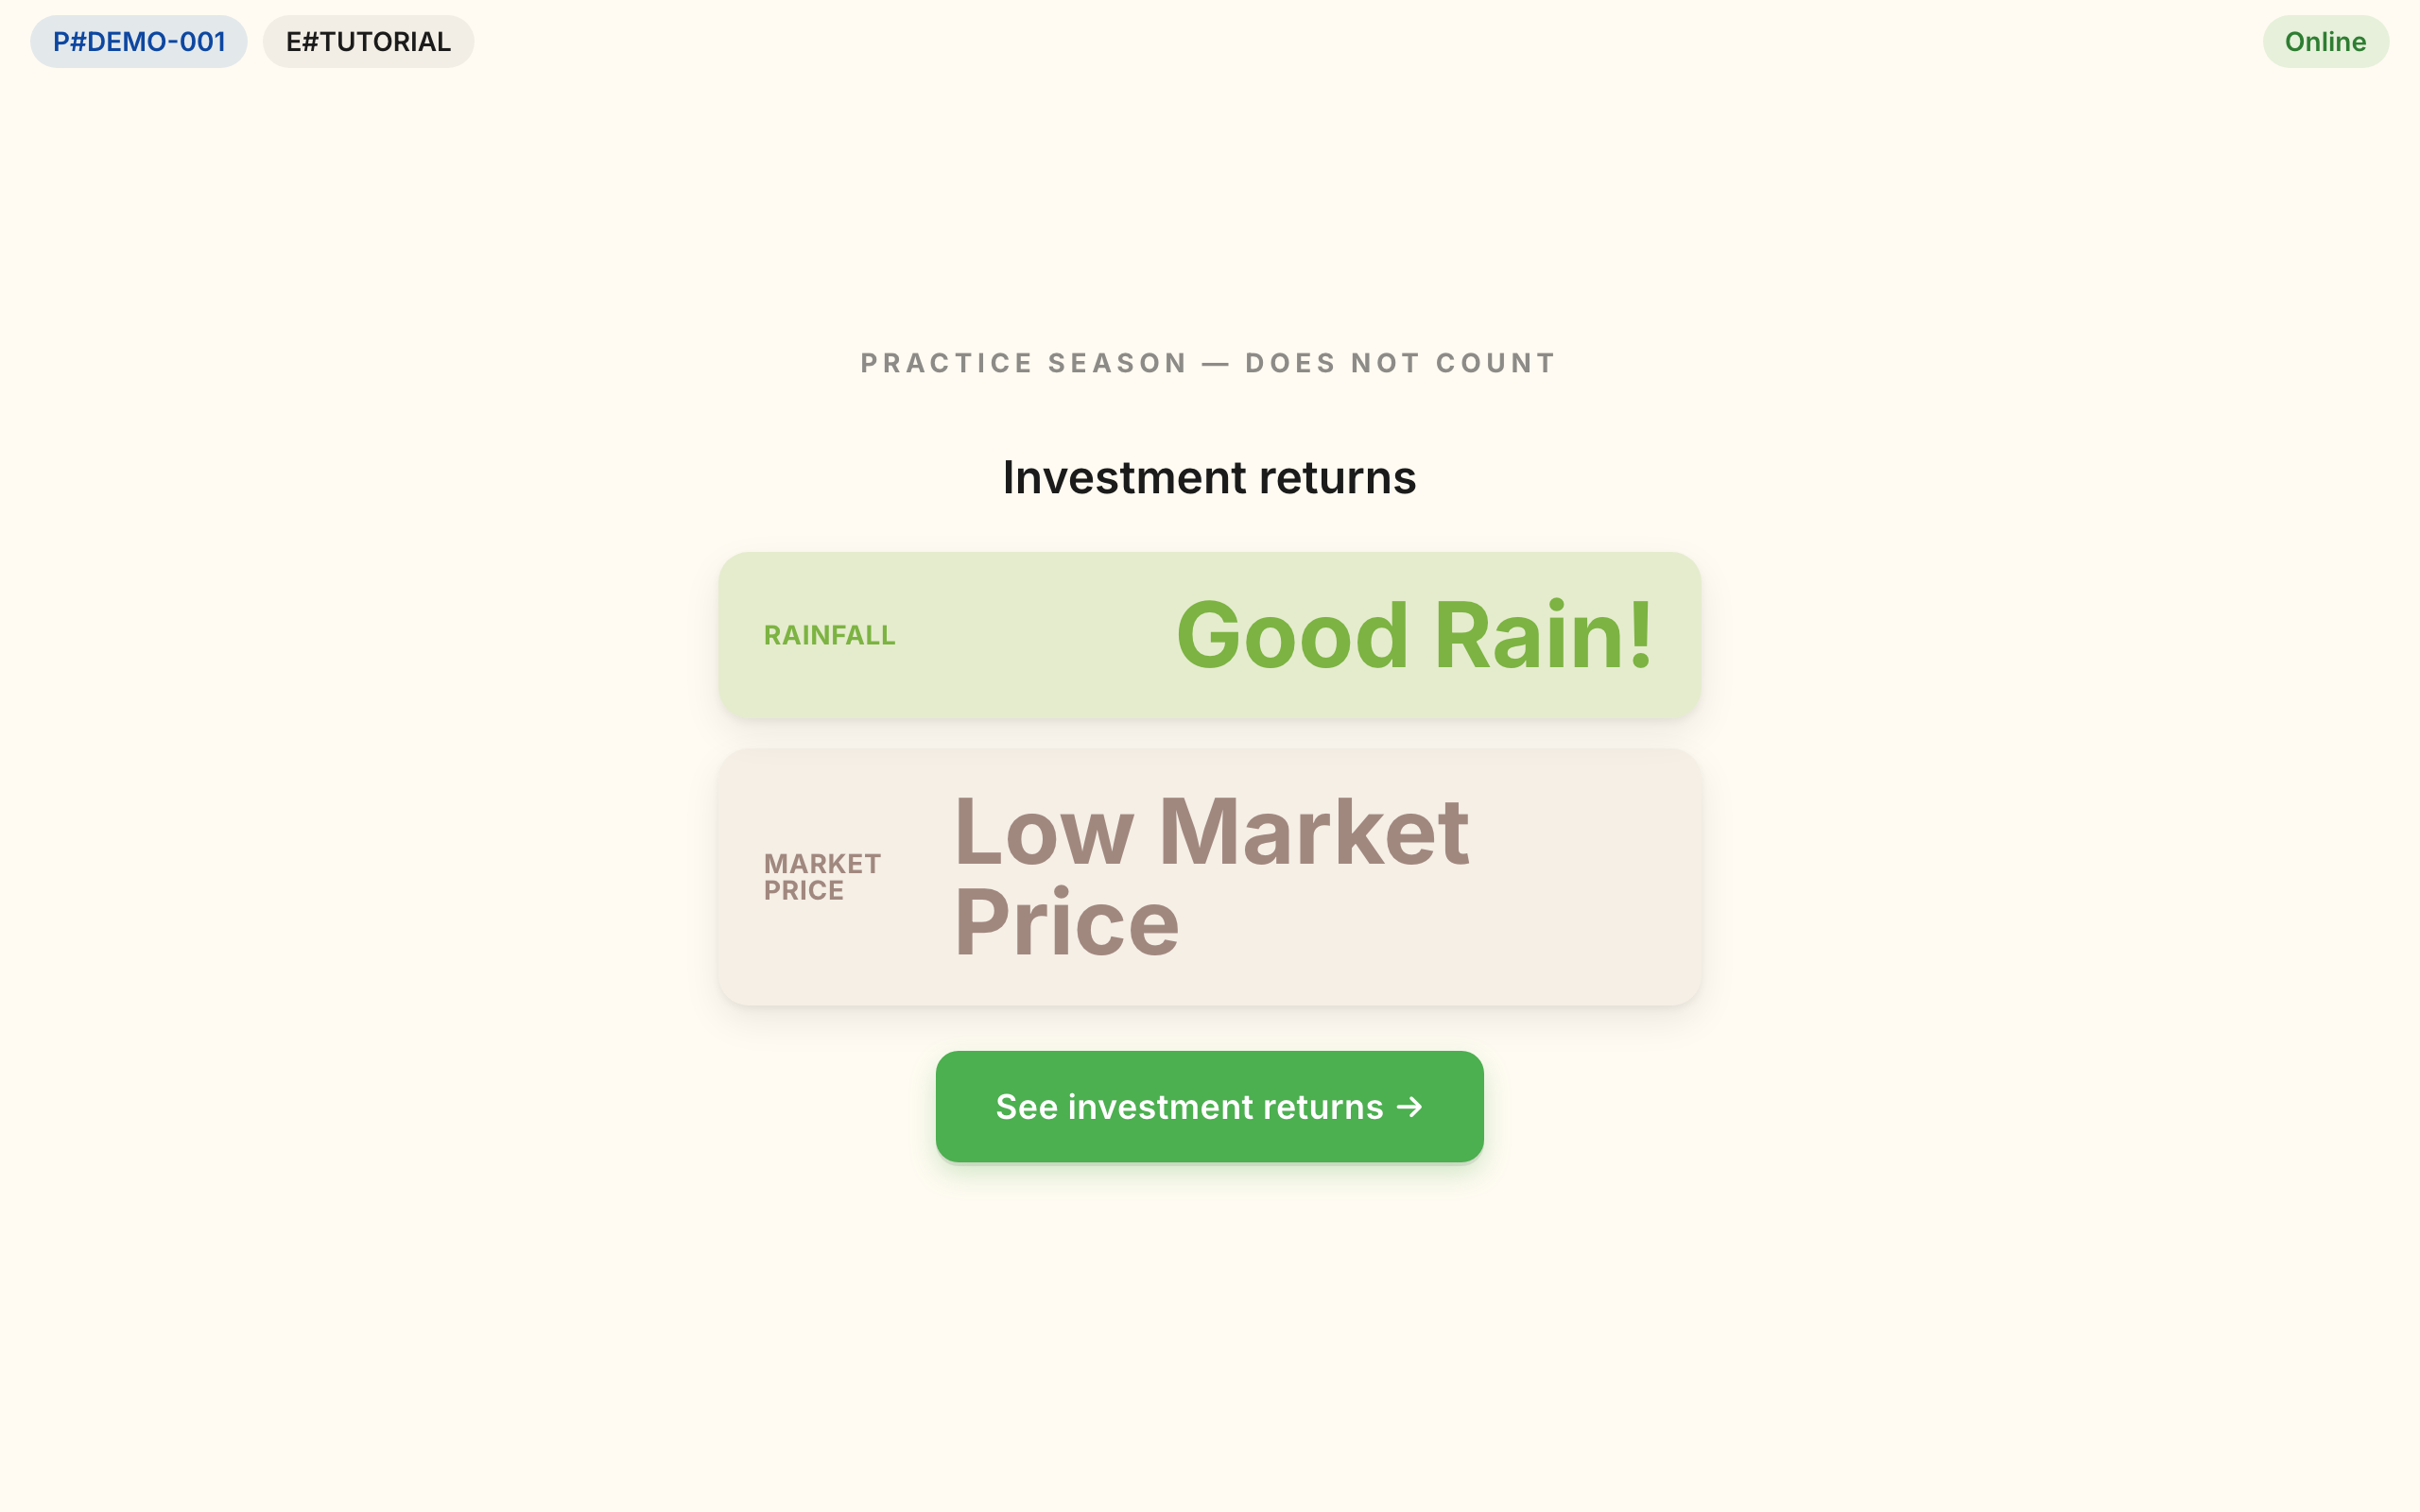
\includegraphics[width=\linewidth]{img/12-reveal-price.png}}\\[2pt]
{\small\itshape\color{inkgrey} Then: the market price.}
\end{minipage}
\end{center}

\subsection{Step 5 --- Your season result}

Finally you see the result of your decision, shown in three simple numbers:

\begin{itemize}[leftmargin=1.4em]
  \item \textbf{Invested in fertilizer} --- the tokens you spent on bags.
  \item \textbf{Net (profit / loss)} --- did the extra harvest earn back \emph{more} than you spent
  (\profit{green, a profit}) or \emph{less} (\loss{brown, a loss})?
  \item \textbf{Take-home} --- the tokens you actually keep this season.
\end{itemize}

\screenshot{img/14-summary-round1.png}{A good season. The farmer invested \textbf{3} bags. The rain was good
and the price was high, so the fertilizer returned \textbf{6.9} tokens --- much more than the 3 invested.
\textbf{Net = \profit{+3.9}}, and take-home is \textbf{28.9} tokens. The game says this in words, too.}

% ===================== 4. THE BIG LESSON =====================
\section{The big lesson: fertilizer can win \emph{or} lose}

The same number of bags can give very different results, depending on the rain and the price.
Below are three real season results from the game.

\subsection{A win --- good rain and high price}
Already shown above: \textbf{invest 3, return 6.9, net \profit{+3.9}}. When the weather and the price are both
good, fertilizer pays off well.

\subsection{Barely worth it --- good rain but low price}

\screenshot{img/13-summary.png}{Here the farmer invested \textbf{6} bags. The harvest grew, but the market
price was \textbf{low}, so the fertilizer only returned \textbf{6.5}. \textbf{Net = \profit{+0.5}}
--- almost exactly break-even. A low price can wipe out your profit.}

\subsection{A loss --- the price did not cover the cost}

\screenshot{img/loss-s2.png}{Here the farmer invested \textbf{9} bags, but the market price was \textbf{low},
so the fertilizer's extra harvest was worth only \textbf{8.5} --- \emph{less} than the 9 invested.
\textbf{Net = \loss{-0.5}}: a loss. Take-home (24.5) is \emph{below} the 25 they started with.}

\warnbox{What a drought does}{%
The worst case is a \textbf{drought}. In a drought, fertilizer does \textbf{nothing} extra --- so the
return is \textbf{0}, and you \textbf{lose every token} you spent on bags. For example, if you buy 8 bags and
a drought comes, your return is 0 and your net is \loss{$-8$}. This is why, when the outlook shows many grey
(drought) squares, buying a lot of fertilizer is risky.}

\keybox{The four cases, in plain words}{%
\begin{tabular}{@{}ll@{}}
\textbf{Good rain {\&} high price} & fertilizer pays off well --- a clear \profit{profit} \\
\textbf{Good rain {\&} low price}  & the harvest is good but sells cheap --- small profit or break-even \\
\textbf{Drought}                   & fertilizer does nothing --- you \loss{lose} what you spent \\
\textbf{Buy no fertilizer}         & you spend nothing and keep all your money --- always safe \\
\end{tabular}}

% ===================== 5. HOW TO THINK =====================
\section{How to decide each season}

There is no single ``correct'' number of bags --- it depends on the chances you are shown. A good way to think:

\begin{enumerate}[leftmargin=1.5em]
  \item \textbf{Look at the rain picture first.} Many green (good) squares and few grey (drought) squares?
  Then fertilizer is more likely to pay off, and buying more makes sense.
  \item \textbf{Then look at the price picture.} Many high/mid squares means your harvest will sell well.
  Many low squares means even a good harvest earns little --- be more careful.
  \item \textbf{When in doubt, buy less.} Buying fewer bags means you risk fewer tokens. Buying \emph{no}
  fertilizer is never a loss.
  \item \textbf{There is no debt.} Even in the worst season you can never go below the tokens you did not
  spend --- you will always take \emph{some} money home.
\end{enumerate}

% ===================== 6. THE WHOLE GAME =====================
\section{The whole game, start to finish}

\begin{enumerate}[leftmargin=1.5em]
  \item A short lesson with pictures, to make sure the rain and price pictures are clear.
  \item \textbf{1 practice season} --- to try the steps. It does \textbf{not} count.
  \item \textbf{10 real seasons} --- each one is the five steps above. Your take-home from each is saved.
  \item \textbf{Final result} --- your tokens from all 10 seasons are added up and changed into real Naira.
\end{enumerate}

\keybox{Remember}{%
Play each season as if the tokens were your own money --- because at the end, they become real money.
Read the pictures, think about the chances, and choose the amount of fertilizer \emph{you} think is worth
the risk.}

\vfill
\begin{center}
{\small\color{inkgrey} CIMMYT Fertilizer Risk-Communication Experiment. Screens shown are the English version;
the game is also played in Hausa. The numbers in the examples are play-tokens.}
\end{center}

\end{document}
